% =====================================================================
%  Seance 4 -- C. cours 3 : optimisation + reponse seance 1 (frames 17--21)
% =====================================================================
\section{Cours 3 --- De la prévision à la décision}

\begin{frame}{Cours 3 --- La chaîne prévision $\to$ marge $\to$ capacité}
\footnotesize%
\begin{center}
\begin{tikzpicture}[node distance=4mm,
  b/.style={draw=byBlue,thick,rounded corners=2pt,fill=byBlue!8,
            minimum height=8mm,text width=2.6cm,align=center,font=\footnotesize},
  a/.style={draw=byOrange,thick,rounded corners=2pt,fill=byOrange!10,
            minimum height=8mm,text width=2.6cm,align=center,font=\footnotesize}]
\node[b] (p) {1. \textbf{Prévision}\\ SARIMA de la charge};
\node[b,right=3mm of p] (m) {2. \textbf{Marge}\\ borne haute 95 \%};
\node[b,right=3mm of m] (c) {3. \textbf{Capacité}\\ CPU, stockage};
\node[a,right=3mm of c] (d) {4. \textbf{Décision}\\ scaler, migrer};
\draw[-{Stealth},thick,byDeep] (p) -- (m);
\draw[-{Stealth},thick,byDeep] (m) -- (c);
\draw[-{Stealth},thick,byDeep] (c) -- (d);
\end{tikzpicture}
\end{center}
\vspace{1mm}
\begin{block}{L'idée clé}
Une prévision \textbf{sans intervalle} ne suffit pas pour dimensionner :
on utilise la \textbf{borne haute} de l'intervalle de confiance (95 \%)
comme marge de sécurité. La MAE mesurée (3,01 pts CPU) dit à quel point
la marge peut être serrée.
\end{block}
\vspace{1mm}
\begin{ebox}[Exemple concret sur le dossier]
Prévision du pic de demain : $p$ pts CPU $\pm$ intervalle. Capacité d'un
serveur : 100 pts. Si la borne haute dépasse la capacité agrégée
$\Rightarrow$ ajouter une instance \textbf{avant} le pic, pas pendant.
\end{ebox}
\end{frame}

\begin{frame}{Autoscaling : décider sans humain dans la boucle}
\begin{columns}[t]
\begin{column}{0.52\textwidth}
\begin{block}{Deux familles de règles}
\begin{itemize}
\item \textbf{Réactif} : seuil observé (CPU $>$ 80 \% pendant 10 min)
$\Rightarrow$ scaler. Simple, mais \textbf{en retard} sur un pic rapide.
\item \textbf{Prédictif} : la prévision SARIMA anticipe le pic de la
période de charge (notre CPU jour 30,2 \% / nuit 10,0 \%) et scale
\textbf{avant}.
\end{itemize}
\end{block}
\begin{kbox}[Où le ML entre]
Le modèle donne la \textbf{trajectoire} (forme + intervalle) ; la
politique de scaling combine prévision + coût : scaler trop tôt coûte
de l'argent inutile, trop tard coûte des incidents --- exactement
l'arbitrage précision/rappel du cours 2.
\end{kbox}
\end{column}
\begin{column}{0.44\textwidth}
\begin{wbox}[Garde-fous obligatoires]
\begin{itemize}
\item Cooldown : ne pas scaler deux fois en 10 min.
\item Bornes min/max d'instances.
\item Journaliser chaque décision : un autoscaler est lui-même un
système à superviser.
\end{itemize}
\end{wbox}
\end{column}
\end{columns}
\end{frame}

\begin{frame}{Date de saturation du stockage : un calcul réel}
\begin{center}
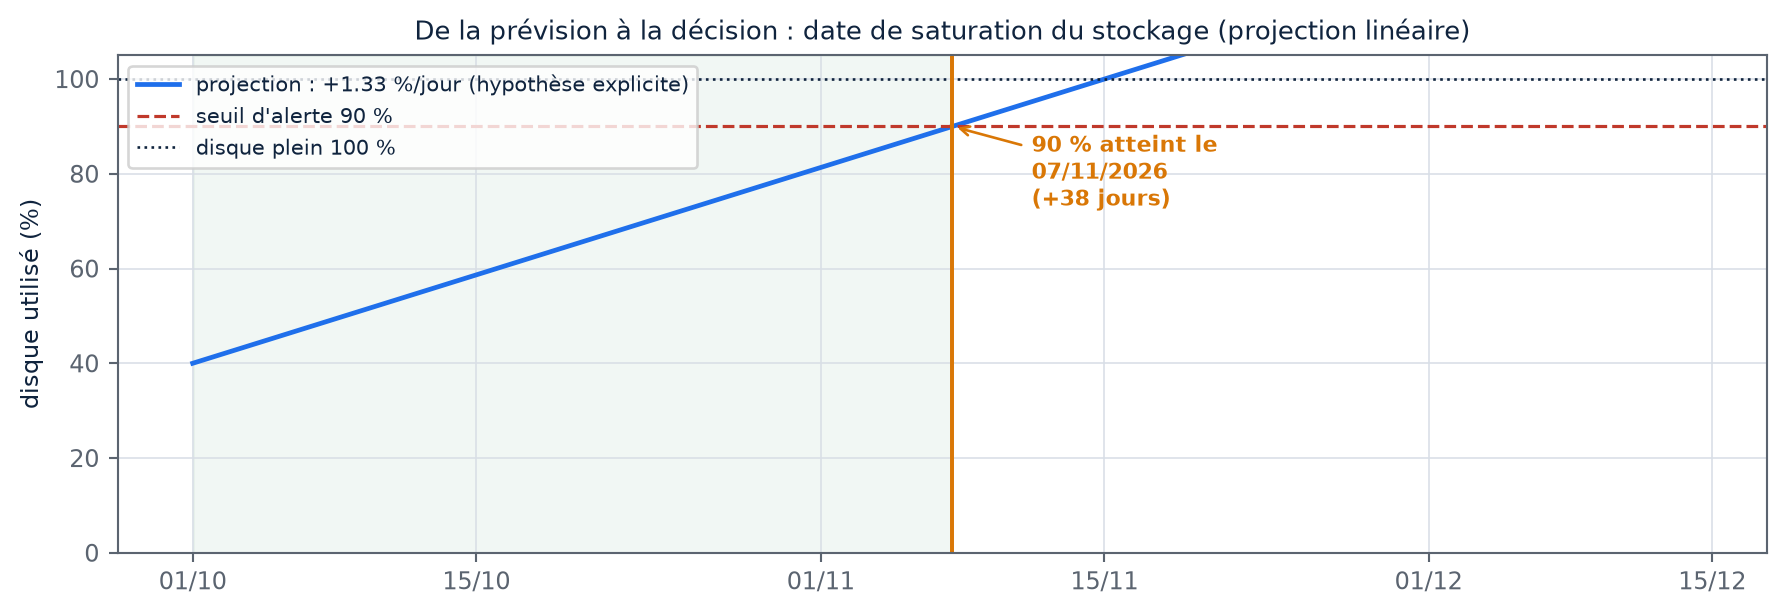
\includegraphics[width=0.88\textwidth]{f28_saturation.png}
\end{center}
\vspace{-1mm}
\begin{columns}[t]
\begin{column}{0.52\textwidth}
\begin{block}{Hypothèses explicites}
\small Métriques + logs : 40 \% du disque après 30 jours de rétention
$\Rightarrow$ \textbf{+1,33 \%/jour} ; seuil d'alerte 90 \%.
\end{block}
\end{column}
\begin{column}{0.44\textwidth}
\begin{solbox}[Calcul]
\small $(90-40)/1{,}333 = 37{,}5$ jours $\Rightarrow$ 90 \% atteint le
\textbf{07/11/2026} ; disque plein début décembre.
\end{solbox}
\end{column}
\end{columns}
\end{frame}

\begin{frame}{La réponse à la question de la séance 1}
\begin{qbox}[La question laissée ouverte en séance 1]
\begin{center}\normalsize
« Si on détectait 70 \% des incidents 30 minutes à l'avance,\\
quelle disponibilité atteindrions-nous ? »
\end{center}
\end{qbox}
\vspace{1mm}
\begin{columns}[t]
\begin{column}{0.52\textwidth}
\begin{block}{Le raisonnement (chiffres du dossier)}
\begin{itemize}
\item indisponibilité cumulée mesurée (séance 1) : \textbf{11,3 h} ;
\item 70 \% évités $\Rightarrow$ indispo restante
$11{,}3 \times 0{,}3 = \mathbf{3{,}39}$ h ;
\item fenêtre de mesure du dossier : $8$ serveurs $\times\ 720$ h
$=$ \textbf{5 760 heures-serveur}.
\end{itemize}
\end{block}
\end{column}
\begin{column}{0.44\textwidth}
\begin{solbox}[Le résultat officiel]
\begin{center}
$\text{dispo} = 1 - \dfrac{3{,}39}{5\,760} = \mathbf{99{,}941\ \%}$
\end{center}
\vspace{1mm}
\textbf{$>$ SLA 99,9 \%} : la détection prédictive n'est pas un
gadget, elle fait \textbf{basculer le parc au-dessus du SLA} --- c'est
la promesse tenue par la partie 4 du syllabus.
\end{solbox}
\end{column}
\end{columns}
\end{frame}

\begin{frame}{Quiz 3 --- optimisation (5 min)}
\begin{qbox}[3 questions]
\begin{enumerate}
\item Pour dimensionner la capacité, on utilise :\\
(a) la moyenne de la prévision \quad (b) la borne haute de l'intervalle
de confiance \quad (c) le maximum historique
\item Le scaling \textbf{prédictif} différend du réactif car :\\
(a) il est gratuit \quad (b) il agit \emph{avant} le pic grâce à la
prévision \quad (c) il ne peut pas se tromper
\item Avec +1,33 \%/jour et 40 \% utilisés, le seuil 90 \% est atteint :\\
(a) après 37,5 jours \quad (b) après 90 jours \quad (c) jamais
\end{enumerate}
\end{qbox}
\vspace{1mm}
\begin{solbox}[Réponses]
\textbf{1 : b} --- la marge vient de l'incertitude mesurée.
\quad \textbf{2 : b} --- et il peut se tromper : d'où les garde-fous.
\quad \textbf{3 : a} --- 50 points à 1,33 point/jour, soit le
07/11/2026.
\end{solbox}
\end{frame}
